\documentclass[11pt]{article}

\usepackage[a4paper,top=22mm,bottom=21mm,left=22mm,right=22mm,headheight=22pt]{geometry}
\usepackage{fontspec}
\usepackage{xeCJK}
\defaultfontfeatures{Ligatures=TeX}
\setmainfont{Latin Modern Roman}
\setsansfont{Lato}
\setmonofont[Scale=0.82]{Noto Sans Mono}
\setCJKmainfont{Noto Serif CJK SC}
\setCJKsansfont{Noto Sans CJK SC}
\setCJKmonofont[Scale=0.82]{Noto Sans Mono CJK SC}
\usepackage{amsmath,amssymb,amsthm,mathtools}
\usepackage{booktabs,array,tabularx}
\usepackage{enumitem}
\usepackage[most]{tcolorbox}
\usepackage{tikz}
\usetikzlibrary{arrows.meta,positioning,calc}
\usepackage{microtype}
\usepackage{fancyhdr}
\usepackage{lastpage}
\usepackage{xcolor}
\usepackage{hyperref}
\usepackage{bookmark}

\definecolor{ArgusNavy}{HTML}{132638}
\definecolor{ArgusBlue}{HTML}{1C6E8C}
\definecolor{ArgusTeal}{HTML}{13A89E}
\definecolor{ArgusGold}{HTML}{D69A2D}
\definecolor{ArgusInk}{HTML}{21313C}
\definecolor{ArgusMuted}{HTML}{61717C}
\definecolor{ArgusPale}{HTML}{EDF4F5}
\definecolor{ArgusWarm}{HTML}{FBF5E8}
\definecolor{ArgusRule}{HTML}{CBD8DC}

\hypersetup{
  colorlinks=true,
  linkcolor=ArgusBlue,
  urlcolor=ArgusBlue,
  citecolor=ArgusBlue,
  pdftitle={A Rank-One Counterexample to the Literal Form of AIM Problem 1.44},
  pdfauthor={Argus Open},
  pdfsubject={All-shell spherical 12-design lattices; Result 20001760},
  pdfkeywords={lattice, spherical design, 12-design, rank one, counterexample, AIM Problem 1.44}
}

\pagestyle{fancy}
\fancyhf{}
\fancyhead[L]{\sffamily\footnotesize\color{ArgusMuted}ARGUS OPEN \enspace/\enspace RESULT 20001760}
\fancyhead[R]{\sffamily\footnotesize\color{ArgusMuted}TECHNICAL REPORT \enspace/\enspace 30 AUGUST 2026}
\fancyfoot[L]{\sffamily\scriptsize\color{ArgusMuted}Open for external mathematical review}
\fancyfoot[R]{\sffamily\scriptsize\color{ArgusMuted}\thepage\ / \pageref*{LastPage}}
\renewcommand{\headrulewidth}{0.4pt}
\renewcommand{\headrule}{\hbox to\headwidth{\color{ArgusRule}\leaders\hrule height \headrulewidth\hfill}}
\renewcommand{\footrulewidth}{0pt}

\setlength{\parindent}{0pt}
\setlength{\parskip}{5.5pt plus 1.2pt minus 1pt}
\setlist[itemize]{leftmargin=5mm,itemsep=2pt,topsep=3pt}
\setlist[enumerate]{leftmargin=6mm,itemsep=2.5pt,topsep=3pt}
\renewcommand{\arraystretch}{1.15}
\emergencystretch=2em

\newcommand{\arguslabel}[1]{\textsf{\footnotesize\bfseries\color{ArgusTeal}\MakeUppercase{#1}}}
\newcommand{\reporturl}{\url{https://open.argusbot.cn/results/20001760/ARGUS_RESULT_20001760_TECHNICAL_REPORT.pdf}}
\newcommand{\artifact}[1]{\texttt{\small #1}}

\newtcolorbox{resultbox}[1][]{
  enhanced,breakable,colback=ArgusPale,colframe=ArgusTeal,
  boxrule=0pt,leftrule=2.2pt,arc=1.5mm,
  left=4mm,right=4mm,top=3mm,bottom=3mm,#1
}
\newtcolorbox{scopebox}[1][]{
  enhanced,breakable,colback=ArgusWarm,colframe=ArgusGold,
  boxrule=0pt,leftrule=2.2pt,arc=1.5mm,
  left=4mm,right=4mm,top=3mm,bottom=3mm,#1
}
\newtcolorbox{notebox}[1][]{
  enhanced,breakable,colback=white,colframe=ArgusRule,
  boxrule=0.5pt,arc=1.5mm,left=4mm,right=4mm,top=3mm,bottom=3mm,#1
}

\newtheoremstyle{argusplain}{5pt}{5pt}{\itshape}{}{\sffamily\bfseries\color{ArgusNavy}}{.}{0.5em}{}
\theoremstyle{argusplain}
\newtheorem{theorem}{Theorem}
\newtheorem{lemma}{Lemma}

\begin{document}

\begin{titlepage}
\thispagestyle{empty}

\begin{tikzpicture}[remember picture,overlay]
  \fill[ArgusNavy] (current page.north west) rectangle ([yshift=-36mm]current page.north east);
  \fill[ArgusTeal] ([yshift=-36mm]current page.north west) rectangle ([yshift=-38.2mm]current page.north east);
  \fill[ArgusPale] ([xshift=151mm,yshift=-180mm]current page.north west) circle (47mm);
  \fill[ArgusTeal,opacity=.10] ([xshift=163mm,yshift=-207mm]current page.north west) circle (32mm);
\end{tikzpicture}

\vspace*{-7mm}
{\sffamily\color{white}\fontsize{10}{12}\selectfont\bfseries ARGUS OPEN}
\hfill
{\sffamily\color{white}\fontsize{9}{11}\selectfont RESULT 20001760 \enspace\textbullet\enspace TECHNICAL REPORT}

\vspace{35mm}

{\arguslabel{Definition-level counterexample}}\\[4mm]
{\sffamily\bfseries\color{ArgusNavy}\fontsize{25}{29}\selectfont
A Rank-One Counterexample\\
to the Literal Form of\\
AIM Problem 1.44\par}

\vspace{5mm}
{\sffamily\color{ArgusMuted}\fontsize{13}{17}\selectfont
Every nonempty shell of $a\mathbb Z$ is the full zero-sphere\\
and hence a spherical $t$-design for every $t$\par}

\vspace{9mm}
\begin{resultbox}
\centering\sffamily
\begin{tabular}{>{\bfseries\color{ArgusNavy}}c@{\hspace{13mm}}>{\bfseries\color{ArgusNavy}}c@{\hspace{13mm}}>{\bfseries\color{ArgusNavy}}c}
rank $1$ & every nonempty shell & all strengths $t$\\[-1mm]
\multicolumn{3}{c}{\color{ArgusTeal}\Large $\displaystyle
L=a\mathbb Z,\quad L_{a^2k^2}=\{-ak,ak\},\quad
\frac{1}{ak}L_{a^2k^2}=S^0$}
\end{tabular}
\end{resultbox}

\vspace{5mm}
\begin{scopebox}
\textsf{\bfseries\color{ArgusNavy}Scope boundary.}
This note refutes only the dimension-unqualified sentence printed as AIM Problem 1.44.
It does not settle a modified problem imposing $n\geq2$ or a narrower lattice class.
No claim of worldwide priority is made.
\end{scopebox}

\vfill
\begin{minipage}[b]{0.59\textwidth}
{\sffamily\bfseries\color{ArgusNavy}中文结论}\par
{\small AIM Problem 1.44 的正式文本没有维数限制。对任意 $a>0$，满一维格 $a\mathbb Z$ 的每个非空正范数壳层归一化后就是整个零维球面 $S^0=\{-1,1\}$，所以对任意强度 $t$ 都是球面 $t$-设计，特别是球面 12-设计。该结论不涉及另加 $n\geq2$ 的修改版本。}
\end{minipage}
\hfill
\begin{minipage}[b]{0.30\textwidth}
\raggedleft\sffamily\small
Prepared by \textbf{Argus Open}\\
30 August 2026\\[2mm]
Independent audit complete
\end{minipage}
\end{titlepage}

\tableofcontents
\vspace{4mm}

\begin{notebox}
\textsf{\bfseries\color{ArgusNavy}Review status.}
The source mapping, counterexample, and atomic audit publication each passed an independent review. The audit root records this item as \artifact{independently\_verified}. This is an open technical report, not a claim of journal peer review.
\end{notebox}

\section{Abstract}

AIM Problem 1.44 asks for a proof that no lattice has every shell a spherical $12$-design. The official HTML, TeX, and PDF versions of the problem impose no dimension restriction. For any $a>0$, take the full rank-one lattice $L=a\mathbb Z\subset\mathbb R$. Every nonempty positive-norm shell of $L$ is a pair $\{-ak,ak\}$; after radial normalization it is exactly the full zero-sphere $S^0=\{-1,1\}$. Its uniform average therefore equals the spherical average for every polynomial, with no degree restriction. Thus every nonempty shell is a spherical $t$-design for every $t$, in particular for $t=12$.

This gives a complete counterexample to the literal dimension-unqualified statement. It does not address the modified problem obtained by adding $n\geq2$. Independent review also confirmed that the frequently cited Leech-lattice $11\tfrac12$-design property is not a $12$-design witness: that notation deliberately skips degree $12$, and the Leech minimum shell is explicitly not a $12$-design.

\section{The exact source statement}

The official problem list for the AIM workshop \emph{Discrete geometry and automorphic forms} prints the following item, attributed to Kumar:

\begin{scopebox}
\centering
\textbf{Problem 1.44.} ``Prove there is no lattice whose shells are spherical $12$-designs.''
\end{scopebox}

The same one-sentence body occurs in the official HTML, TeX, and PDF exports. None of them states a lower bound on dimension or rank, or imposes integrality, parity, unimodularity, or self-duality.

The database label attached to the audited input had created a source-mapping trap: the number $98$ in the AimPL aggregate data is the ordering position of the entire problem list, not a problem number. The target itself is Problem 1.44. A different Problem 1.32 appears on the same aggregate page but is mathematically unrelated. The audit recovered the complete item before deciding the claim.

\section{Definitions}

Let $L\subset\mathbb R^n$ be a full lattice. For $m>0$, its norm-$m$ shell is
\[
  L_m=\{x\in L:\langle x,x\rangle=m\}.
\]
As usual in all-shell design statements, the property concerns nonempty positive-norm shells. If $L_m\neq\varnothing$, its radial normalization is the finite subset
\[
  X_m=m^{-1/2}L_m\subset S^{n-1}.
\]

A nonempty finite set $X\subset S^{n-1}$ is a spherical $t$-design if, for every polynomial $P$ of degree at most $t$,
\[
  \frac1{|X|}\sum_{x\in X}P(x)
  =\int_{S^{n-1}}P(x)\,d\sigma(x),
\]
where $\sigma$ is normalized rotation-invariant measure. This is the standard averaging definition used in the lattice-design literature \cite{VenkovMartinet,Pache2005}.

In dimension one,
\[
  S^0=\{-1,1\},
  \qquad
  \int_{S^0}P(x)\,d\sigma(x)=\frac{P(-1)+P(1)}2.
\]
No harmonic-polynomial equivalence theorem is needed below: the normalized shell will be the entire sphere itself.

\section{The counterexample}

\begin{theorem}[Rank-one witness]
For every real $a>0$, every nonempty positive-norm shell of the lattice $L=a\mathbb Z\subset\mathbb R$ is a spherical $t$-design for every nonnegative integer $t$. Consequently, $L$ is a counterexample to the literal form of AIM Problem 1.44.
\end{theorem}

\textit{Proof.}
Fix $m>0$ with $L_m\neq\varnothing$. Then $m=a^2k^2$ for some integer $k\geq1$, and the only lattice vectors of norm $m$ are
\[
  L_m=\{-ak,ak\}.
\]
Since $\sqrt m=ak$, radial normalization gives
\[
  X_m=m^{-1/2}L_m=\{-1,1\}=S^0.
\]
Therefore for every polynomial $P$, without any degree restriction,
\[
  \frac1{|X_m|}\sum_{x\in X_m}P(x)
  =\frac{P(-1)+P(1)}2
  =\int_{S^0}P(x)\,d\sigma(x).
\]
Thus $X_m$ is a spherical $t$-design for every $t$, including $t=12$. The argument applies to every nonempty positive-norm shell of $a\mathbb Z$. \hfill$\square$

\begin{figure}[ht]
\centering
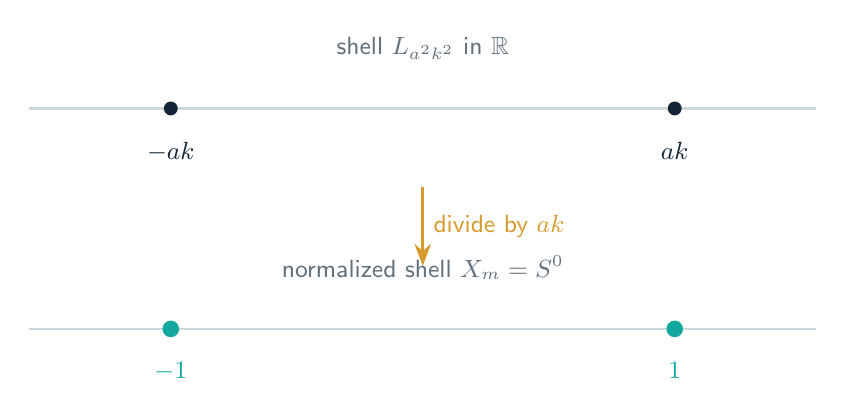
\begin{tikzpicture}[>=Stealth,every node/.style={font=\sffamily\small}]
  \draw[ArgusRule,line width=1pt] (-5,0)--(5,0);
  \fill[ArgusNavy] (-3.2,0) circle (2.5pt) node[below=3mm] {$-ak$};
  \fill[ArgusNavy] (3.2,0) circle (2.5pt) node[below=3mm] {$ak$};
  \node[above=5mm,text=ArgusMuted] at (0,0) {shell $L_{a^2k^2}$ in $\mathbb R$};
  \draw[->,ArgusGold,line width=1.1pt] (0,-1.0)--(0,-2.0) node[midway,right] {divide by $ak$};
  \draw[ArgusRule,line width=1pt] (-5,-2.8)--(5,-2.8);
  \fill[ArgusTeal] (-3.2,-2.8) circle (3pt) node[below=3mm] {$-1$};
  \fill[ArgusTeal] (3.2,-2.8) circle (3pt) node[below=3mm] {$1$};
  \node[above=5mm,text=ArgusMuted] at (0,-2.8) {normalized shell $X_m=S^0$};
\end{tikzpicture}
\caption{Every nonempty shell of $a\mathbb Z$ becomes the complete zero-sphere after radial normalization.}
\end{figure}

The special choice $a=1$ gives $L=\mathbb Z$, which is integral and self-dual. Thus even adding either of those two unstated adjectives would not remove the witness; an explicit exclusion of rank one would.

\section{Why the Leech-lattice lead does not decide the problem}

Pache proves that all shells of the Leech lattice are spherical $11\tfrac12$-designs \cite{Pache2005}. This notation is not an ordinary strength between $11$ and $12$. For an antipodal set, an $11\tfrac12$-design satisfies the even harmonic conditions in degrees
\[
  2,4,6,8,10,14,
\]
whereas a spherical $12$-design requires the conditions in degrees
\[
  2,4,6,8,10,12.
\]
The half-strength notation deliberately skips degree $12$ and adds degree $14$. Moreover, the proof immediately preceding Pache's Theorem 32 states that the Leech minimum shell cannot be a $12$-design. The Leech lattice is therefore not an all-shell $12$-design counterexample.

This correction matters because the audited input initially carried only the Leech $11\tfrac12$-design lead. The decisive argument instead comes directly from the unqualified dimension in the official AIM statement and the rank-one lattice $a\mathbb Z$.

\section{Independent review and audit publication}

The result passed two separate review gates:

\begin{enumerate}
  \item An independent mathematical Reviewer recovered the full AIM item from the official HTML, TeX, PDF, and a historical page; checked that no dimension qualifier was hidden in the surrounding text; verified the $S^0$ averaging identity; and accepted the counterexample with the explicit $n\geq2$ limitation.
  \item A fresh integration Reviewer independently checked the atomic publication. The previous $297$ audit rows remained byte-identical, the only new ID was 20001760, all scientific fields matched the accepted staging row, and only \artifact{review\_status} was promoted to \artifact{independently\_verified}.
\end{enumerate}

The resulting audit root contains $298$ unique reviewed IDs and has SHA-256
\begin{resultbox}
\centering\ttfamily\small
94a5d11151a1a877d4bc367c476a5b8bacb44244b4ee3d9001ac6a43d29639ea
\end{resultbox}

\subsection{Exact production timeline}

All times below are UTC on 30 August 2026.

\begin{center}
\begin{tabularx}{\textwidth}{@{}l l X@{}}
\toprule
Time & Elapsed & Milestone\\
\midrule
04:55:05 & 00:00:00 & Source-recovery and rank-one-counterexample mission started.\\
05:21:39 & 00:26:34 & Engineer completed the source map, proof, evidence package, and staging row.\\
05:28:27 & 00:33:22 & Independent mathematical Reviewer accepted the literal counterexample.\\
05:33:06 & 00:38:01 & Separate atomic-publication mission started.\\
05:41:18 & 00:46:13 & The single-row atomic replacement completed with persisted transaction evidence.\\
05:50:06 & 00:55:01 & Fresh integration Reviewer accepted the published 298-row root.\\
\bottomrule
\end{tabularx}
\end{center}

Thus the mathematical result reached independent acceptance in approximately \textbf{33 minutes}; the end-to-end path through independently reviewed publication took approximately \textbf{55 minutes}. Much of that time was source-identity recovery and audit verification. Once the unrestricted wording was established, the mathematical witness itself was immediate.

\section{Scope and significance}

\subsection{What is proved}

The exact sentence printed as AIM Problem 1.44 is false: a full rank-one lattice has every nonempty shell a spherical $12$-design. The proof is exact, self-contained, and does not depend on numerical search.

\subsection{What is not proved}

\begin{scopebox}
\begin{itemize}
  \item No conclusion is claimed for a repaired statement requiring dimension or rank at least two.
  \item No classification of higher-dimensional all-shell design lattices is claimed.
  \item The report does not claim that the likely intended higher-dimensional problem is easy or resolved.
  \item No worldwide-priority or novelty claim is made.
\end{itemize}
\end{scopebox}

The result is best viewed as a precise formulation correction backed by a complete counterexample. Its natural scale is a short technical note: mathematically decisive for the literal wording, but deliberately limited in scope.

\clearpage
\section{External review checklist}

An external reviewer can check the complete argument in a few steps:
\begin{enumerate}
  \item Read the complete official body of AIM Problem 1.44 and verify that it contains no dimension restriction.
  \item Confirm that $a\mathbb Z$ is a full rank-one lattice in $\mathbb R$.
  \item For every nonempty positive-norm shell, derive $L_{a^2k^2}=\{-ak,ak\}$.
  \item Normalize by $ak$ and verify that the resulting set is exactly $S^0=\{-1,1\}$.
  \item Compare the uniform two-point average with normalized spherical measure on $S^0$.
  \item Keep the literal statement separate from a proposed $n\geq2$ variant.
  \item Do not substitute the Leech $11\tfrac12$-design property for a $12$-design claim.
\end{enumerate}

\phantomsection
\addcontentsline{toc}{section}{References}
\small
\begin{thebibliography}{9}
\setlength{\itemsep}{2pt}

\bibitem{AIM144}
American Institute of Mathematics,
\emph{Discrete Geometry and Automorphic Forms: Problem 1.44},
official AimPL HTML, TeX, and PDF problem-list exports.
\url{http://aimpl.org/discreteaf/}

\bibitem{VenkovMartinet}
Boris Venkov, notes by Jacques Martinet,
``Réseaux et designs sphériques'' [``Lattices and Spherical Designs''],
Definition 3.1 and surrounding discussion.

\bibitem{Pache2005}
Claude Pache,
``Shells of Selfdual Lattices Viewed as Spherical Designs,''
\emph{International Journal of Algebra and Computation} \textbf{15} (2005), nos.~5--6, 1085--1127.
\url{https://doi.org/10.1142/S0218196705002797}

\end{thebibliography}

\vfill
\begin{notebox}
\centering\sffamily\small
\textbf{Result 20001760} \enspace\textbullet\enspace Shareable report: \reporturl\\
Prepared 30 August 2026 \enspace\textbullet\enspace Comments and independent checks are welcome.
\end{notebox}

\end{document}
